% !TEX root = ../main.tex
\subsection{Preprocessing and feature engineering}

\texttt{data\_preprocessing.ipynb} turns the raw crawl into the catalog through the steps in
Figure~\ref{fig:funnel}. First, only questions with at least one of the 179 curated AI/ML tags are kept,
which removes 95.5\% of the crawl and keeps results on topic. Closed questions are then removed, since
they are off-topic, unclear or point to another question. The text is cleaned by unescaping HTML,
replacing links and images with \texttt{<URL>} and \texttt{<IMG>} tokens, removing leftover HTML tags,
normalising Unicode (NFKC) and collapsing whitespace. Non-English posts are removed with
\texttt{langdetect}, because the embedding model was trained on English. Finally, questions with a body
shorter than 50 characters or with no answers are dropped, so every result the app returns has an answer.
Listing~\ref{lst:clean} shows the cleaning step and the construction of the lower-cased model input.

\begin{figure}[H]
  \centering
  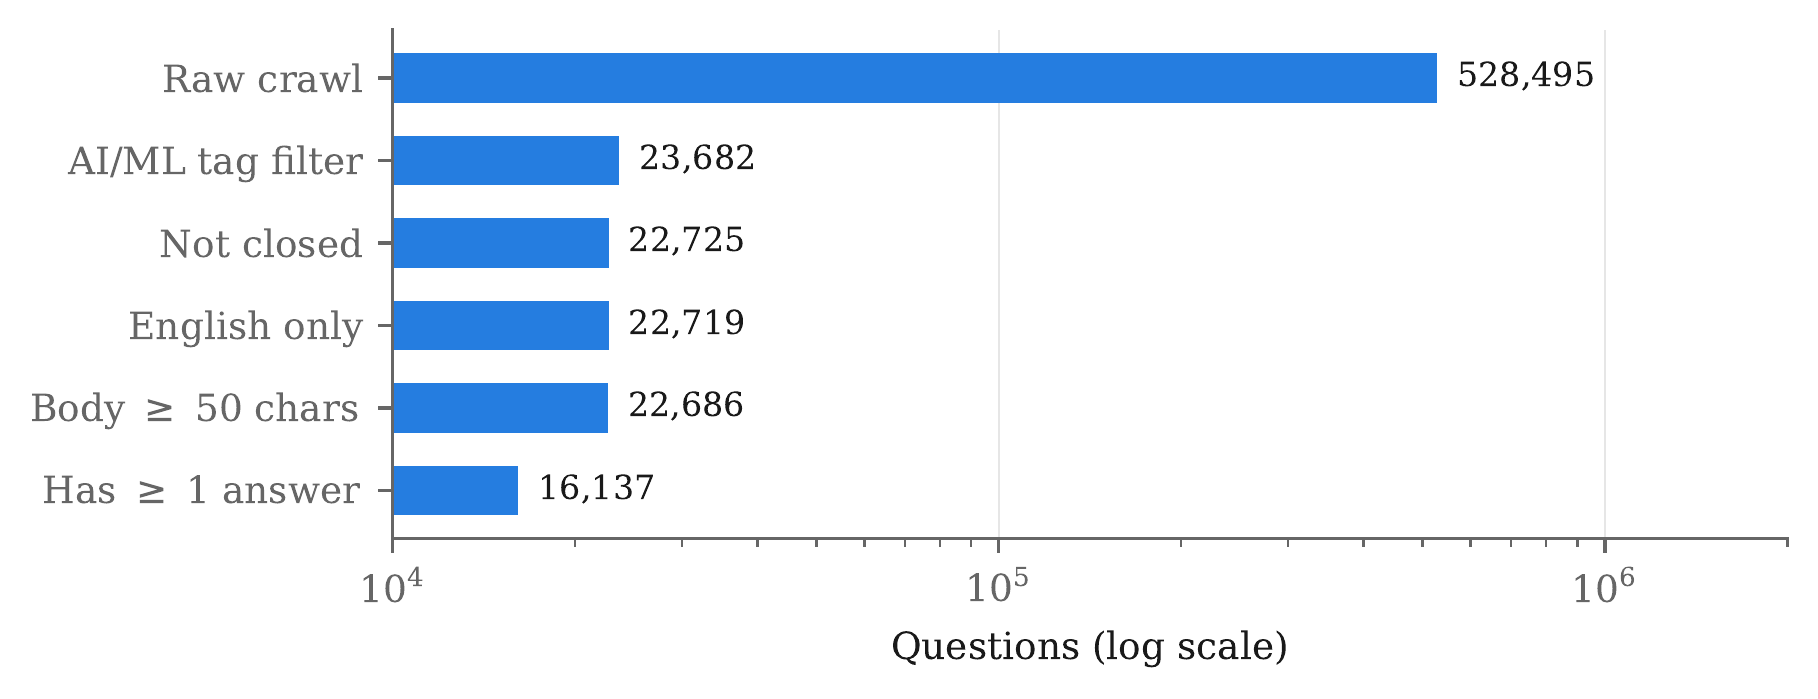
\includegraphics[width=0.78\linewidth]{figures/funnel.png}
  \caption{Questions remaining after each preprocessing step (log scale).}
  \label{fig:funnel}
\end{figure}

\notebooklisting{snippets/clean_text.py}{Text cleaning and construction of the lower-cased model input (\texttt{data\_preprocessing.ipynb})}{lst:clean}

The model input is the lower-cased title and body. Code blocks are left out because long stack traces
and boilerplate would dominate the vectors and hide the actual problem. Two representations are built
from this text. The first is TF-IDF over word 1--2-grams combined with character 3--5-grams, using
sublinear term frequency; the character n-grams match identifiers such as \texttt{OutOfMemoryError} even
when they are split differently (Listing~\ref{lst:vectorizer}). The second is a 384-dimensional sentence embedding. For evaluation only,
each question also keeps its set of AI/ML tags (1.55 per question on average, Figure~\ref{fig:tags}).

\notebooklisting{snippets/tfidf_vectorizer.py}{Building the TF-IDF representation: word and character n-grams joined by \texttt{FeatureUnion} (\texttt{train\_model.ipynb})}{lst:vectorizer}

\begin{figure}[H]
  \centering
  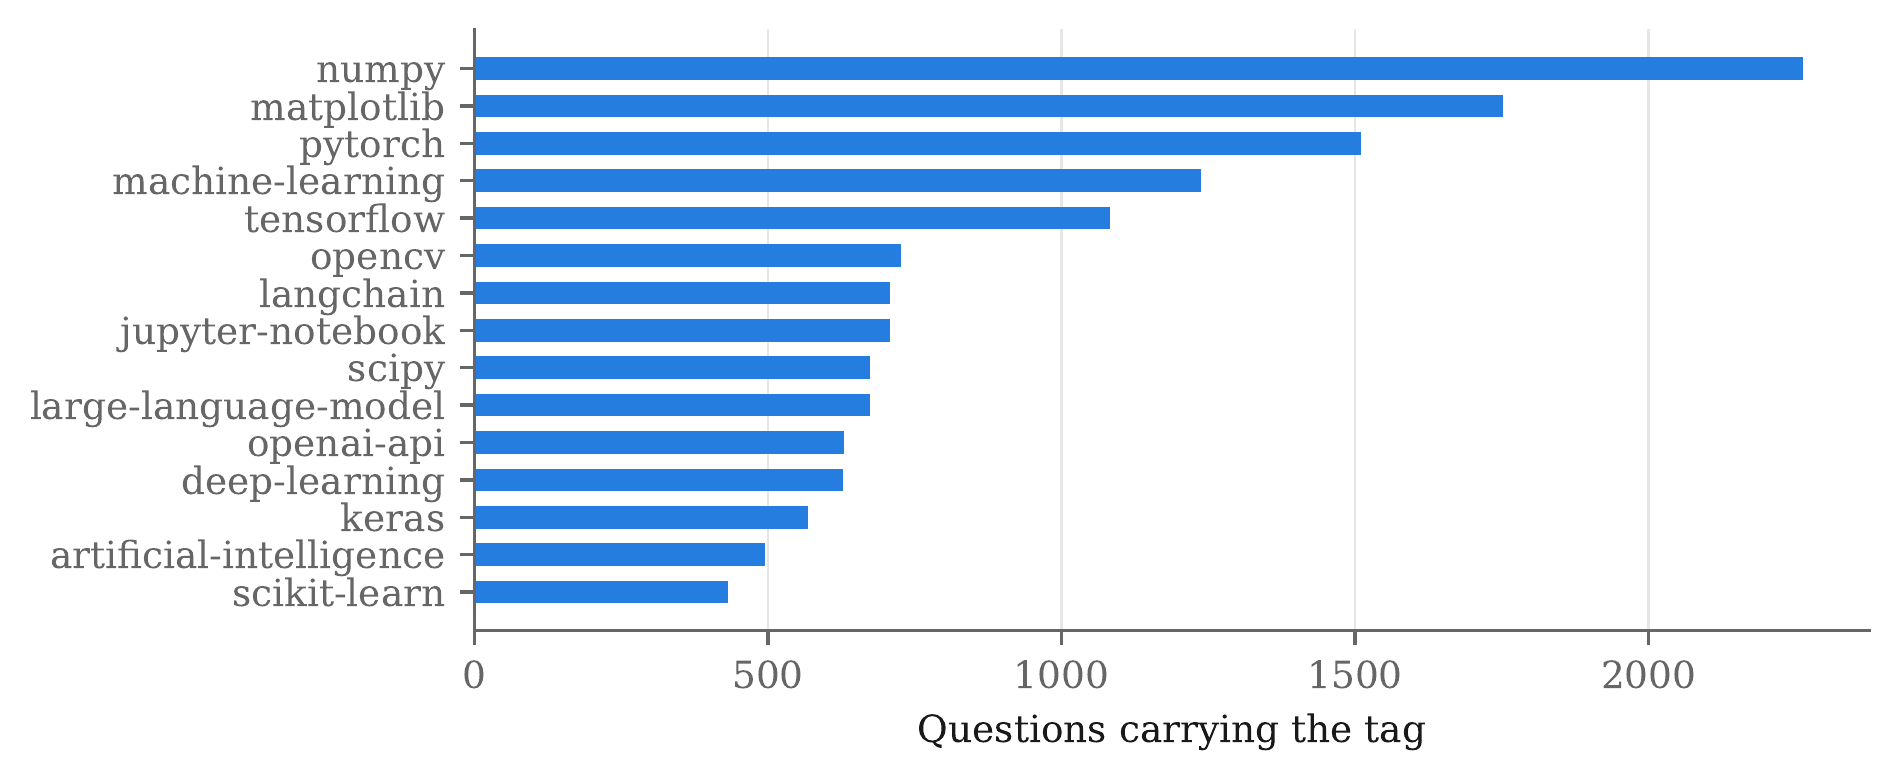
\includegraphics[width=0.7\linewidth]{figures/tags.png}
  \caption{Most frequent AI/ML tags in the 16,137-question catalog.}
  \label{fig:tags}
\end{figure}
